\section{RESULTS AND DISCUSSION}%
\label{chap:Results and Discussion}

The workload evaluations are run multiple times for consistency of results. 
For each workload we give a brief overview of the performance gain 
achieved by the Dyanmic window. 

\subsection{Workload for latency measurement}%
\label{sec:Results Workload for latency measurement}
For latency, Tumbling window has a median value of 1915ms, 
with latency ranging from 1081ms to 2624ms (Figure~\ref{fig:constant_tumb_boxplot})
more than $10\times$ the lantency of Dynamic window, which has a median 
of 57 and ranging from 39 to 120ms (Figure~\ref{fig:constant_dynamic_boxplot}). 
Our improvement to fire the \emph{trigger} event whenever a
new record arrives inside the 
subwindow, allows 
Dynamic window to achieve sub second latency. 

Dynamic window has a 
steady throughput of around 17200 records per second whereas Tumbling window fluctuates between 
12500 and 12800 records per second before stabilizing at 12750 records per second (Figure~\ref{fig:constant_thorughput}). 
This is due to the adjustment of window sizes at the subwindow level, allowing Dynamic window to wait for more records 
with infrequent \emph{key} attribute in the stream, before evicting the subwindow. 
In contrast, Tumbling window 
always evicts the content of the window after 2 seconds without waiting for more 
records.

Relative memory usage of Dynamic window compared to Tumbling window 
is similar over the lifetime of the 
evaluation run (Figure~\ref{fig:constant_mem_diff}). 
Dynamic window causes infrequent \emph{spikes} in memory usage of over
100 MB more than Tumbling window at a certain point in the lifetime of evaluation. 
This can be attributed 
to the subwindows of Dynamic window growing larger due to the low stream 
rate. However,
Dynamic window stabilizes to a more optimal 
window size, where it uses less memory than Tumbling windows. 
At worst case, it uses as much memory as Tumbling window does over the course of the evaluation. 

CPU usage is higher by around 7\% for Dynamic window since it requires extra processing of the calculation of metrics and 
it increases the throughput causing RMLStreamer to process more joined records.
(Figure~\ref{fig:constant_cpu}). 

\begin{figure}[htbp]
    \begin{subfigure}[b]{0.5\columnwidth}
        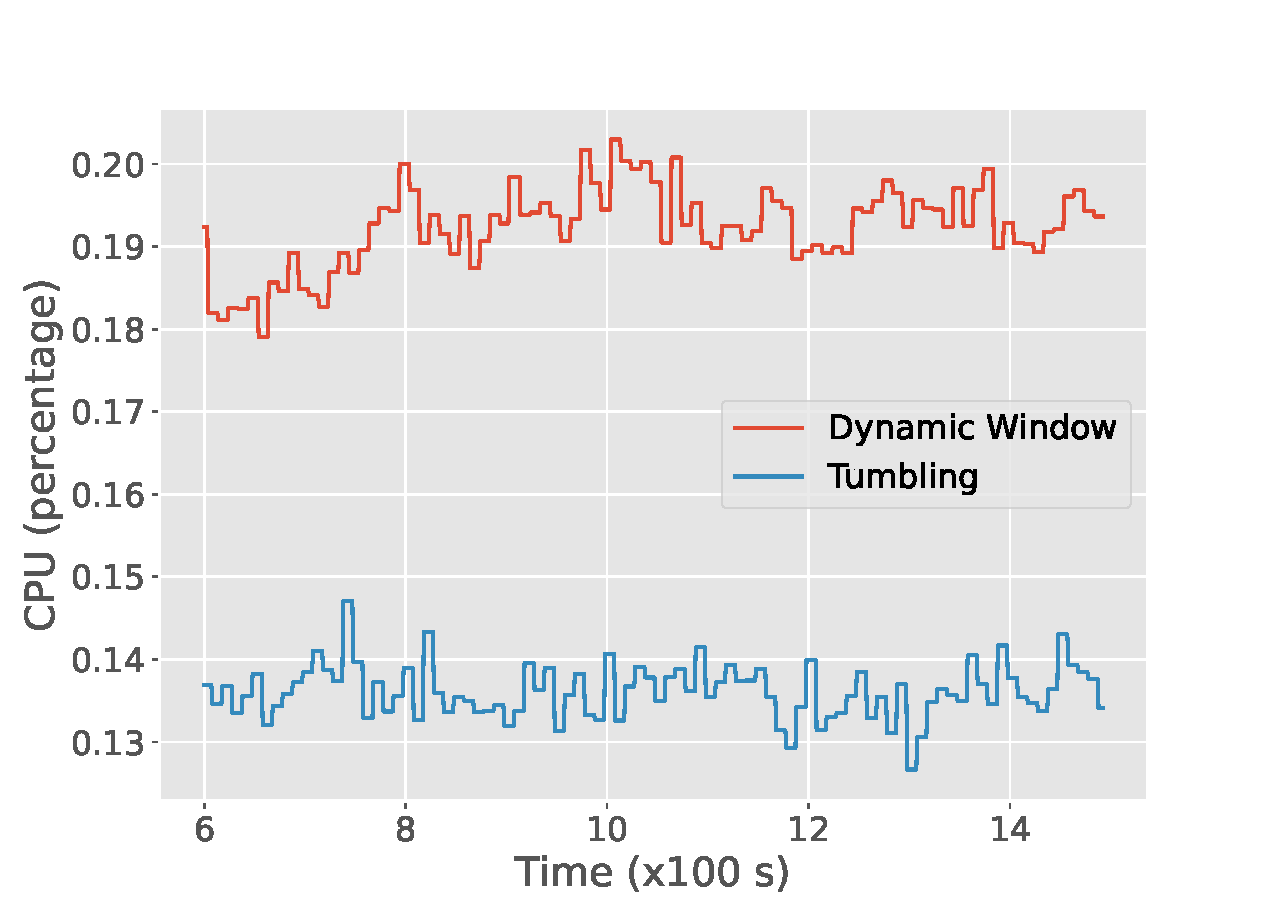
\includegraphics[width=\columnwidth]{fig/constant-rate/cpu_comparison.pdf}
        \caption{CPU usage}
        \label{fig:constant_cpu}
    \end{subfigure}
    \begin{subfigure}[b]{0.5\columnwidth}
        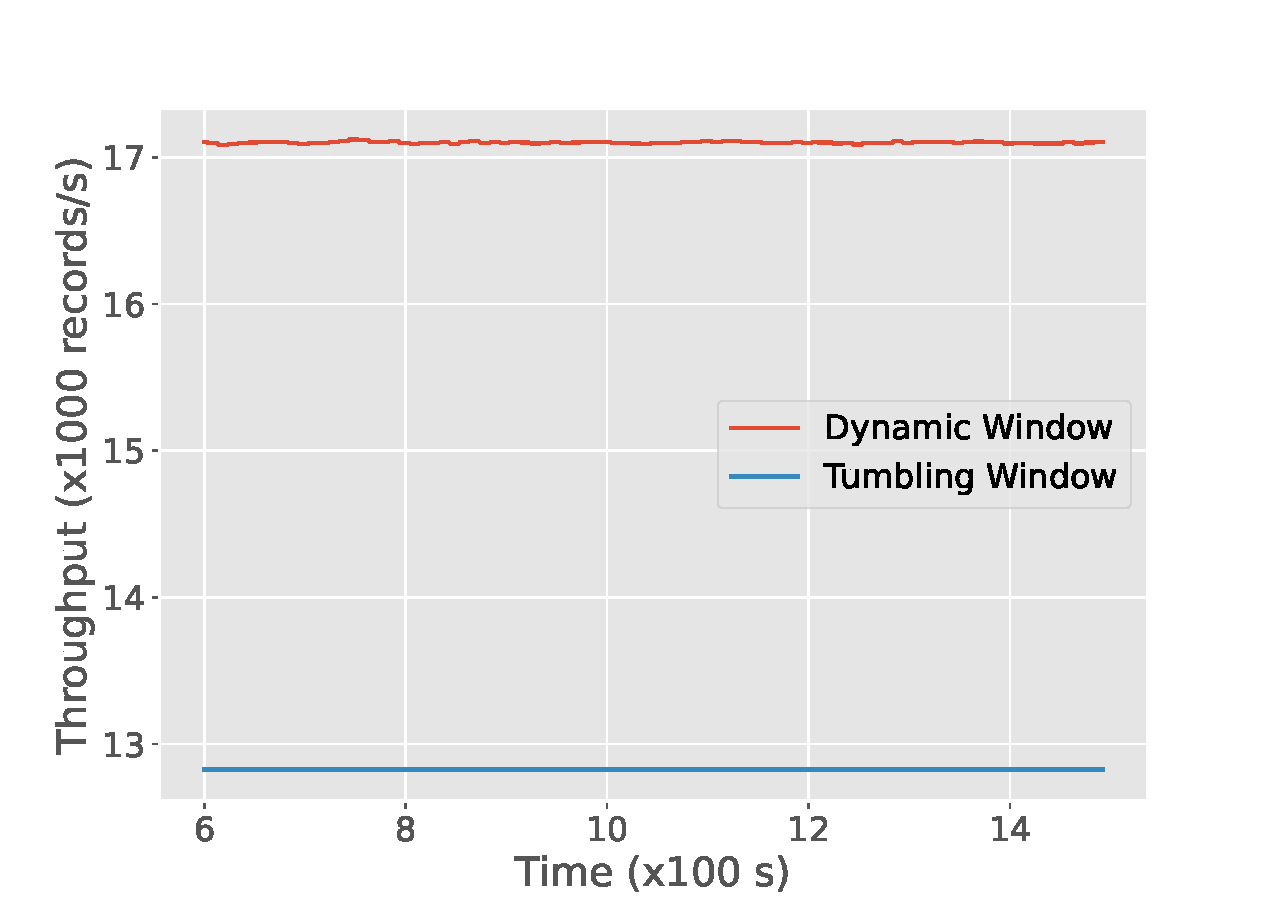
\includegraphics[width=\columnwidth]{fig/constant-rate/throughput_comparison.pdf}
        \caption{Throughput}
        \label{fig:constant_thorughput}
    \end{subfigure}
    %%
    \\
    \begin{subfigure}[b]{0.5\columnwidth}
        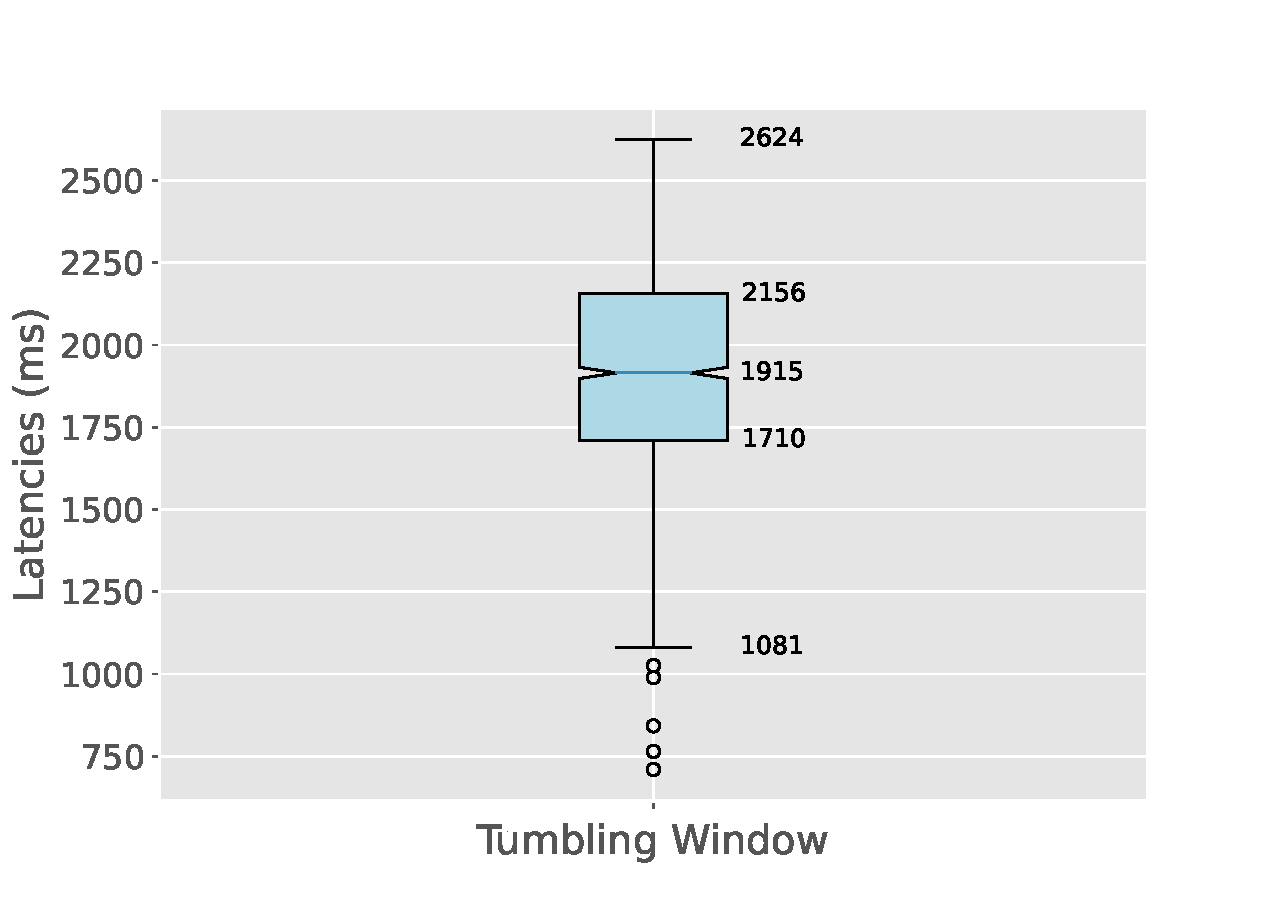
\includegraphics[width=\columnwidth]{fig/constant-rate/TumblingWindow_latency_boxplot.pdf}
        \caption{Tumbling latency}
        \label{fig:constant_tumb_boxplot}
    \end{subfigure}
    \begin{subfigure}[b]{0.5\columnwidth}
        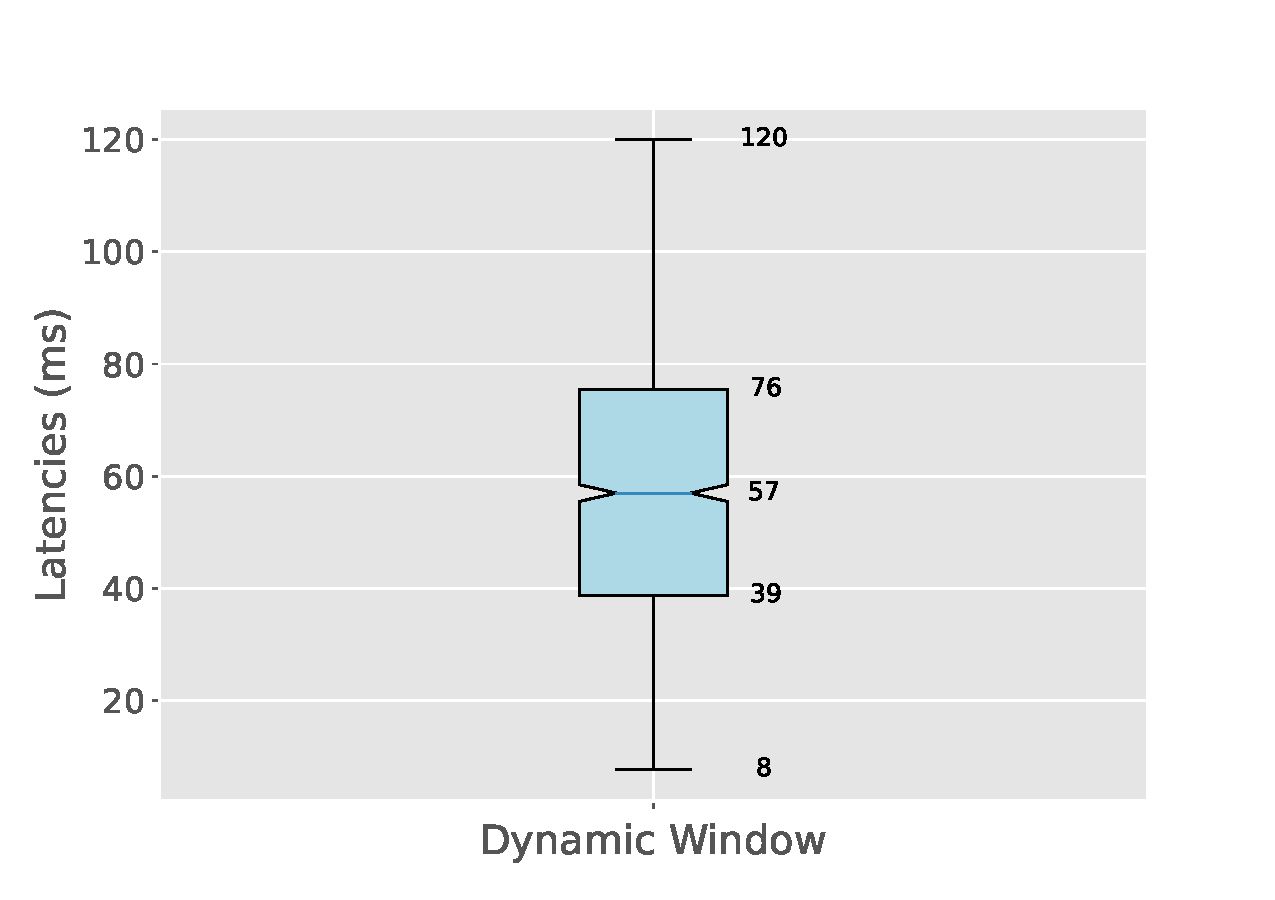
\includegraphics[width=\columnwidth]{fig/constant-rate/DynamicWindow_latency_boxplot.pdf}
        \caption{Dynamic latency}
        \label{fig:constant_dynamic_boxplot}
    \end{subfigure}
    % \\
    \\
    \begin{subfigure}[b]{\columnwidth}
        \centering
        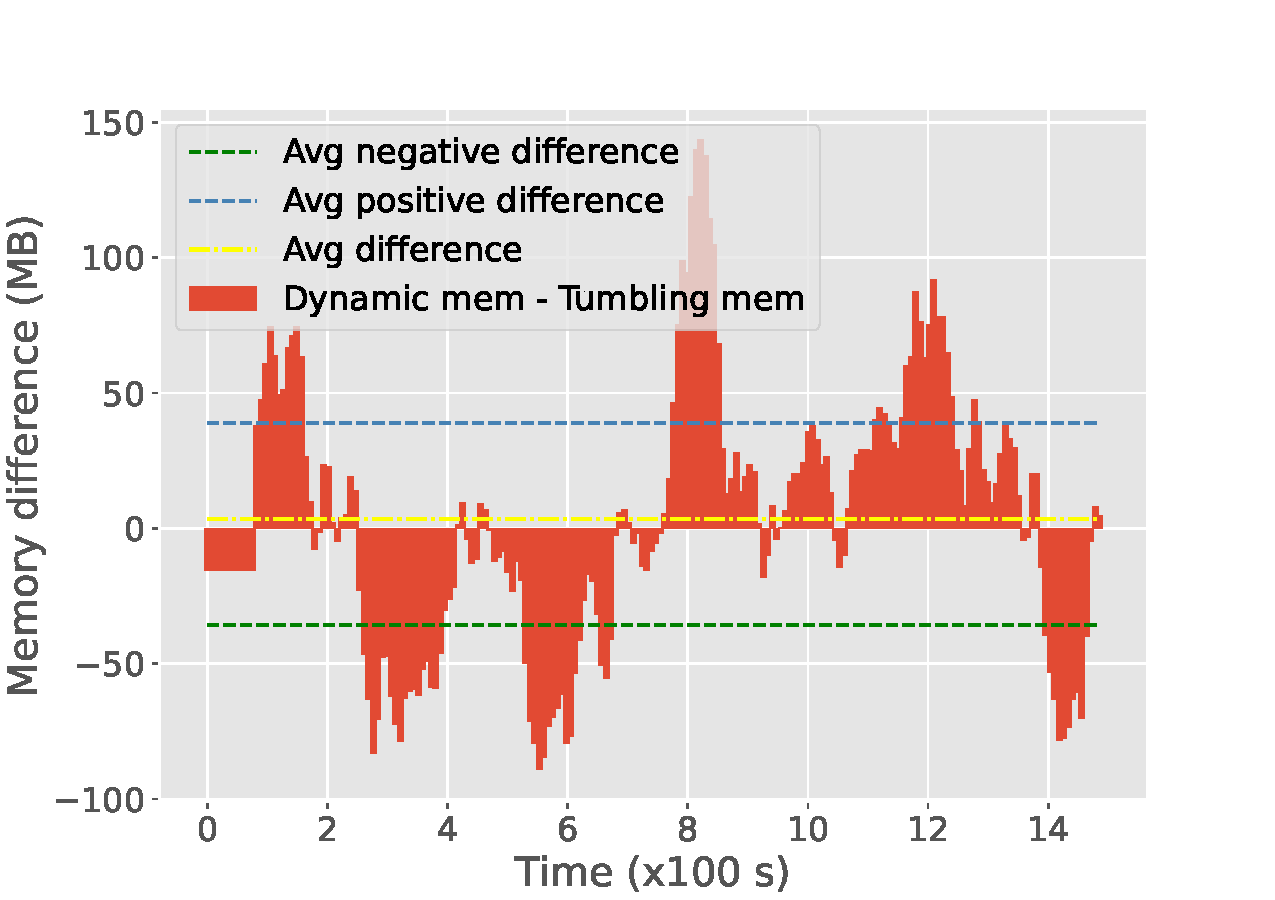
\includegraphics[width=0.5\columnwidth]{fig/constant-rate/mem_difference_bar.pdf}
        \caption{Relative difference in memory usage from the perspective of dynamic window}
        \label{fig:constant_mem_diff}
    \end{subfigure}

    \caption[Metrics measurements for latency workload.]
    {Metrics measurements for latency workload. Dynamic window performs 
    better in all measurements with the exception of CPU usage due to
overhead in dynamic adjustment of subwindow sizes.}%
    \label{fig:constant_measurement}
\end{figure}

\subsection{Workload for periodic burst}%
\label{sec:Results Workload for periodic burst}

Dynamic window still handles the periodic burst of data with lower latency 
than Tumbling window with latency in the range from 8ms to 1669ms
(Figure~\ref{fig:periodic_dynamic_boxplot}) compared to 
Tumbling window's range from 891ms to 3904ms 
(Figure~\ref{fig:periodic_tumb_boxplot}) which is double the latency 
measured for Dynamic window.
However, there is a temporary increase in latency at the beginning 
(Figure~\ref{fig:periodic_dynamic_lineplot}), 
when the burst of data arrives at every 10th second. 
This is due to the initial size of 2s subwindows for the initial low stream rate of 400 records per second. 
The subwindow sizes start to grow \textbf{larger} than 2s because of the low stream rate. 
The increase in the subwindow size results in the 
window having more records to join; causing a back pressure to form and latency to increase.  
This results in a positive skew in the latency distribution for Dynamic window (Figure~\ref{fig:periodic_dynamic_boxplot}). 
However, Dynamic window eventually manages to shorten the subwindow sizes as an
adaptation to the periodic burst of data until it achieves sub second latency again.


The throughput of both windows increased as expected.
Moreover, we observe a bigger difference in the throughput between the 
two windows of about 6000 records per second 
(Figure~\ref{fig:periodic_throughput}). However, the
constant and flat throughput measurement does not agree 
with the results of ~\cite{evalution_of_spe} where there are clear "spikes" in 
the throughput measurement which correspond to the periodic burst 
of records processed by the windows. 
We ran our evaluation as part of the whole RMLStreamer pipeline, causing 
a slight back pressure 
leading to a high and flat throughput measurement. 

CPU usage difference of the windows, is similar to the 
workload for latency measurement with relative increase for 
burst data procesing
(Figure~\ref{fig:periodic_cpu}). 

Surprisingly,
Dynamic window uses 
about 10 MB less memory on average than Tumbling window during the lifetime of the evaluation (Figure~\ref{fig:periodic_mem_diff}). 
The initial memory usage for Dynamic window is about 100 MB higher than for 
Tumbling window due to the long window growth 
caused by the low stream rate. However, once 
the dynamic adjustment of subwindow kicks in, reducing the memory usage.


\begin{figure}
    \begin{subfigure}[b]{\columnwidth}
        \centering
        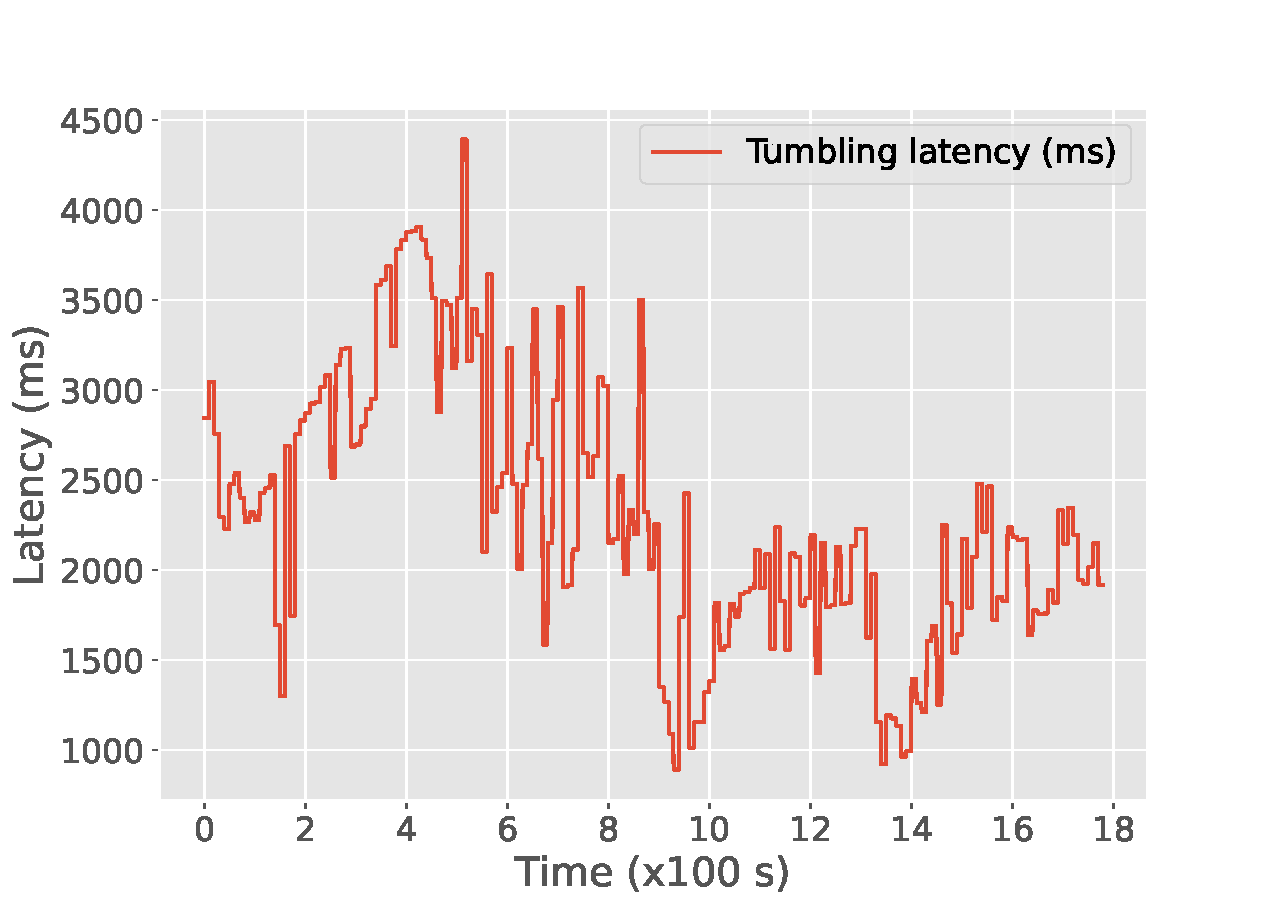
\includegraphics[width=\columnwidth, scale=4]{fig/periodic/Tumbling_latency_lineplot.pdf}
        \caption{Tumbling latency }
        \label{fig:periodic_tumbling_lineplot}
    \end{subfigure}

    \begin{subfigure}[b]{\columnwidth}
        \centering
        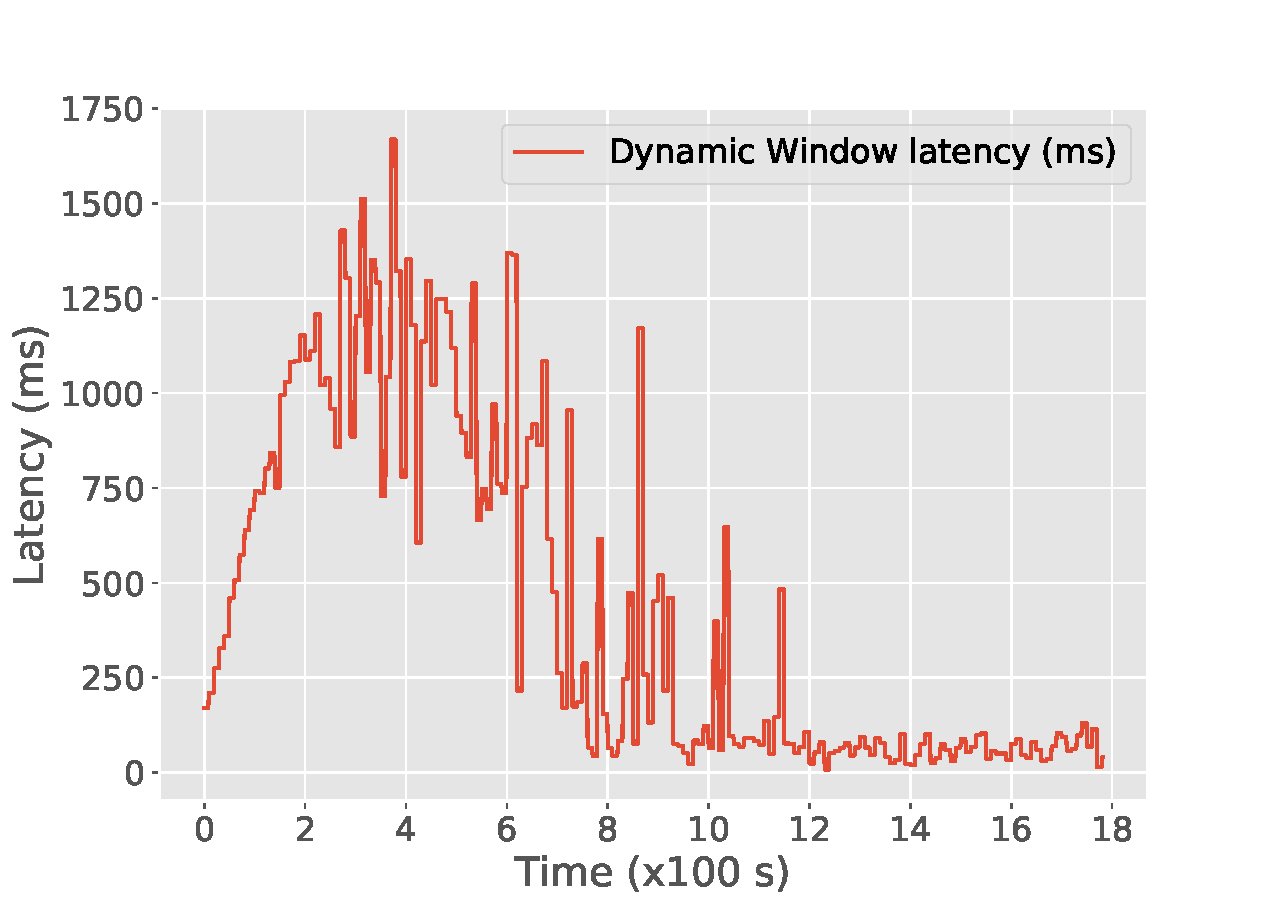
\includegraphics[width=\columnwidth]{fig/periodic/DynamicWindow_latency_lineplot.pdf}
        \caption{Dynamic latency }
        \label{fig:periodic_dynamic_lineplot}
    \end{subfigure}
    \caption{Latency measurement of periodic workload over the lifetime of evaluation}
    \label{fig:periodic_latency_lineplot}
\end{figure}

\begin{figure}
    \begin{subfigure}[b]{0.5\columnwidth}
        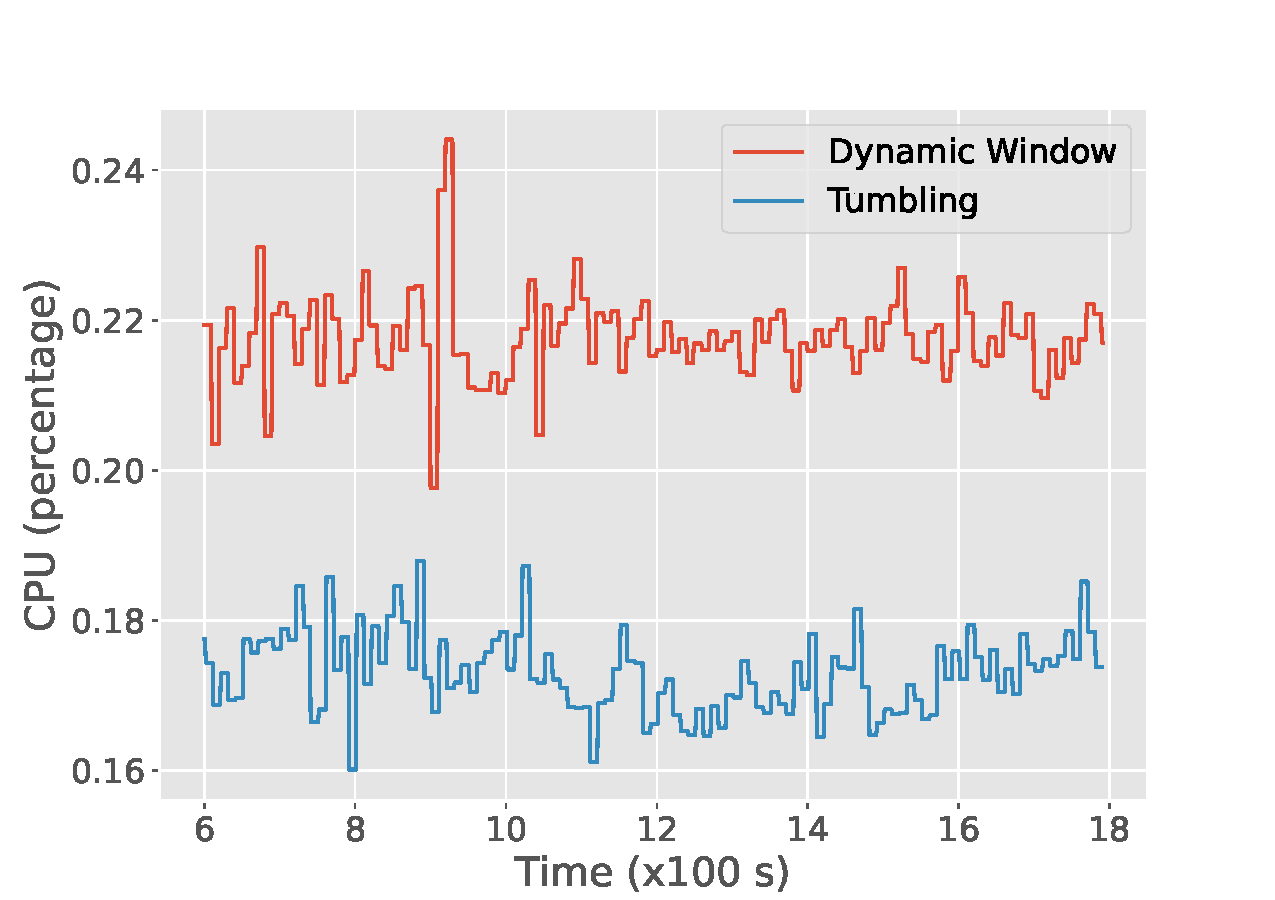
\includegraphics[width=\columnwidth]{fig/periodic/cpu_comparison.pdf}
        \caption{CPU usage}
        \label{fig:periodic_cpu}
    \end{subfigure}
    \hfill 
    \begin{subfigure}[b]{0.5\columnwidth}
        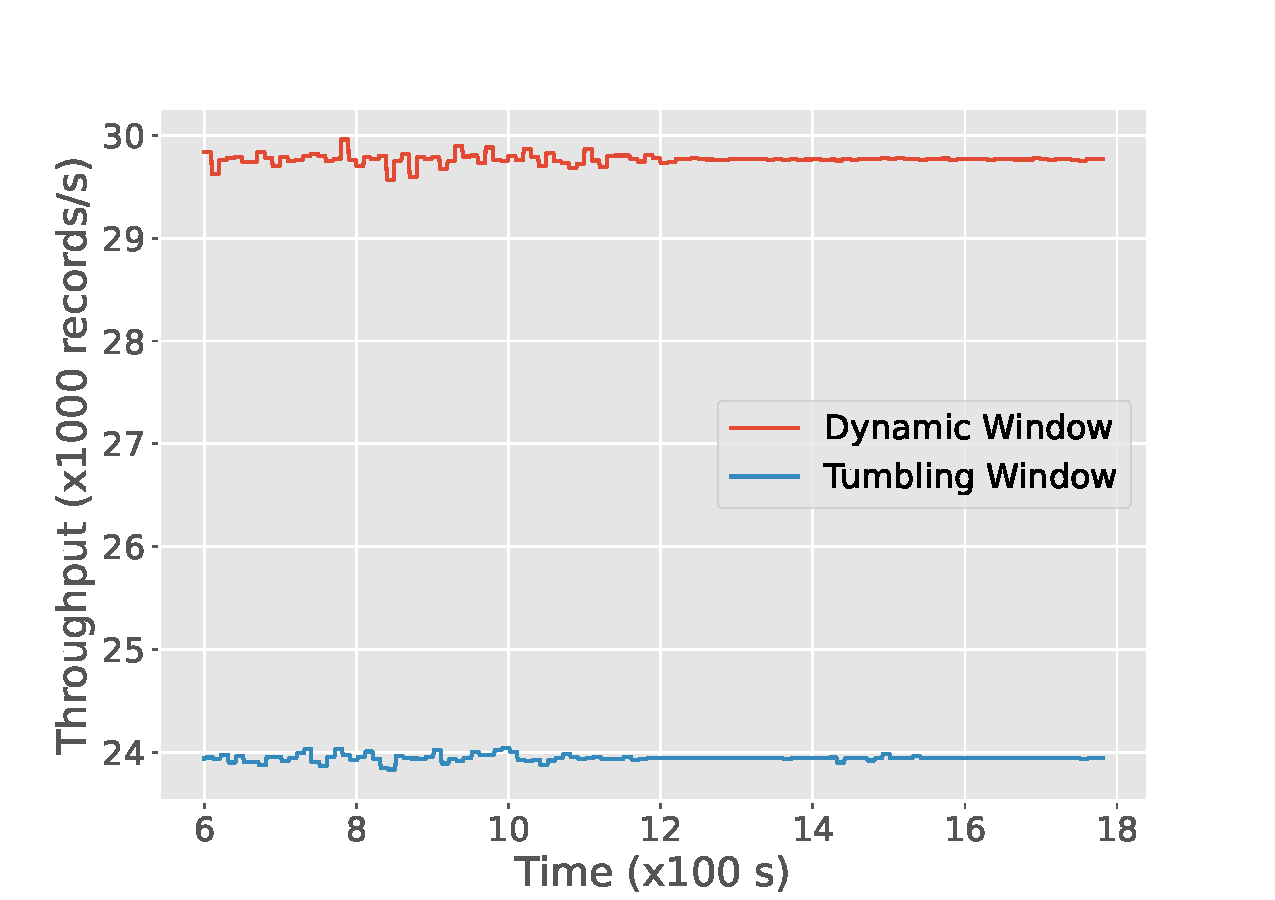
\includegraphics[width=\columnwidth]{fig/periodic/throughput_comparison.pdf}
        \caption{Throughput }
        \label{fig:periodic_throughput}
    \end{subfigure}
    %%
    \begin{subfigure}[b]{0.5\columnwidth}
        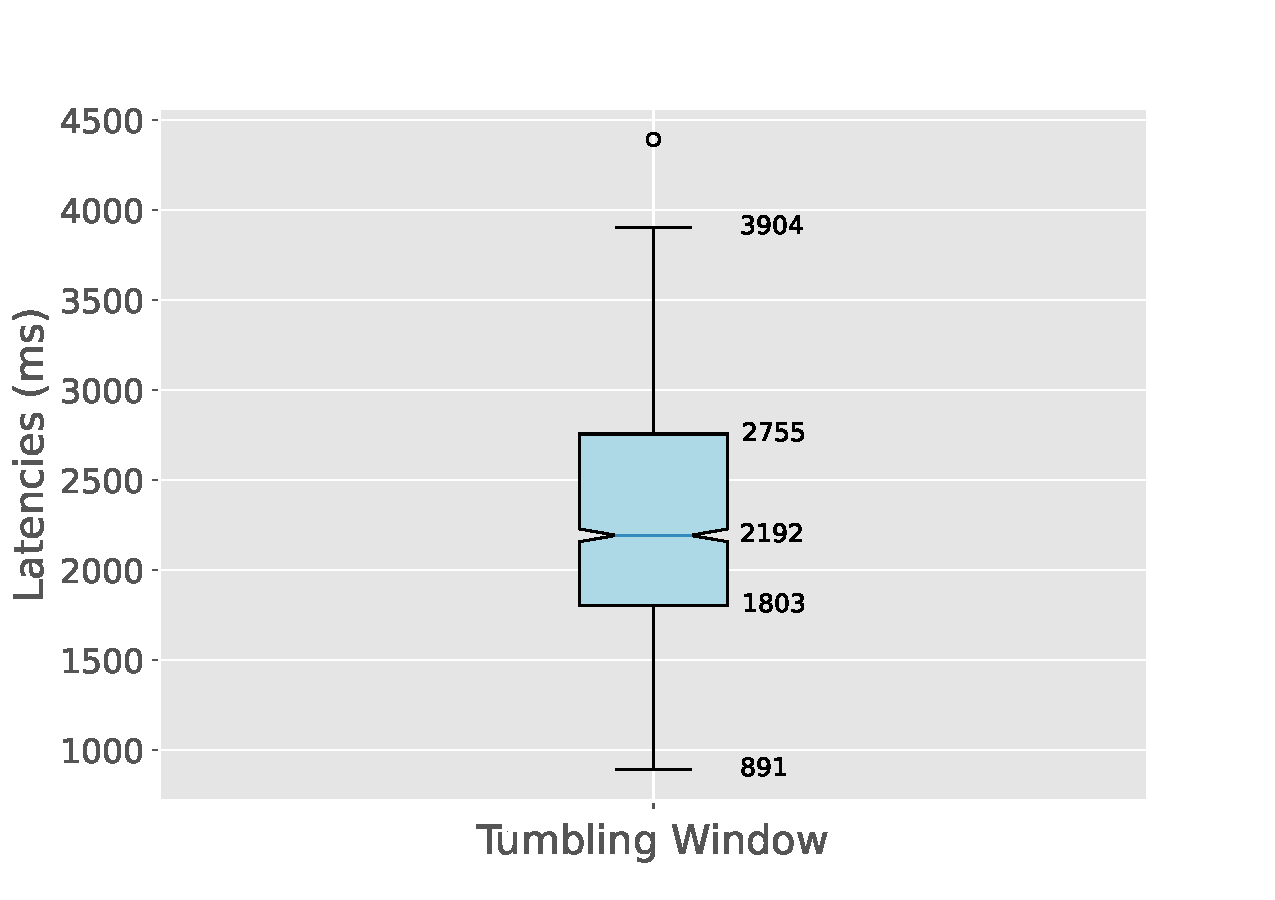
\includegraphics[width=\columnwidth]{fig/periodic/TumblingWindow_latency_boxplot.pdf}
        \caption{Tumbling latency distribution}
        \label{fig:periodic_tumb_boxplot}
    \end{subfigure}
    \hfill 
    \begin{subfigure}[b]{0.5\columnwidth}
        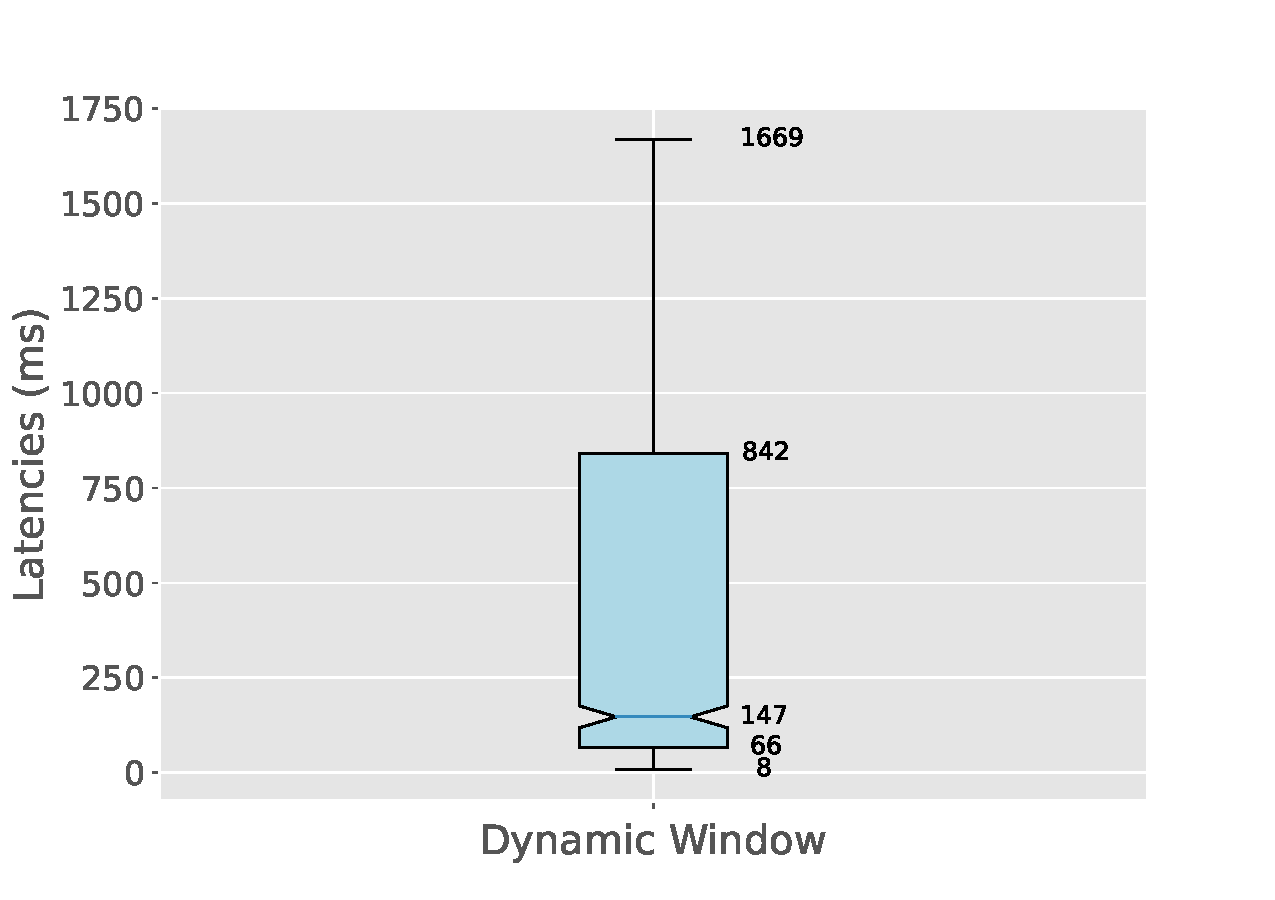
\includegraphics[width=\columnwidth]{fig/periodic/DynamicWindow_latency_boxplot.pdf}
        \caption{Dynamic latency distribution}
        \label{fig:periodic_dynamic_boxplot}
    \end{subfigure}
    % 
    \begin{subfigure}[b]{\columnwidth}
        \centering
        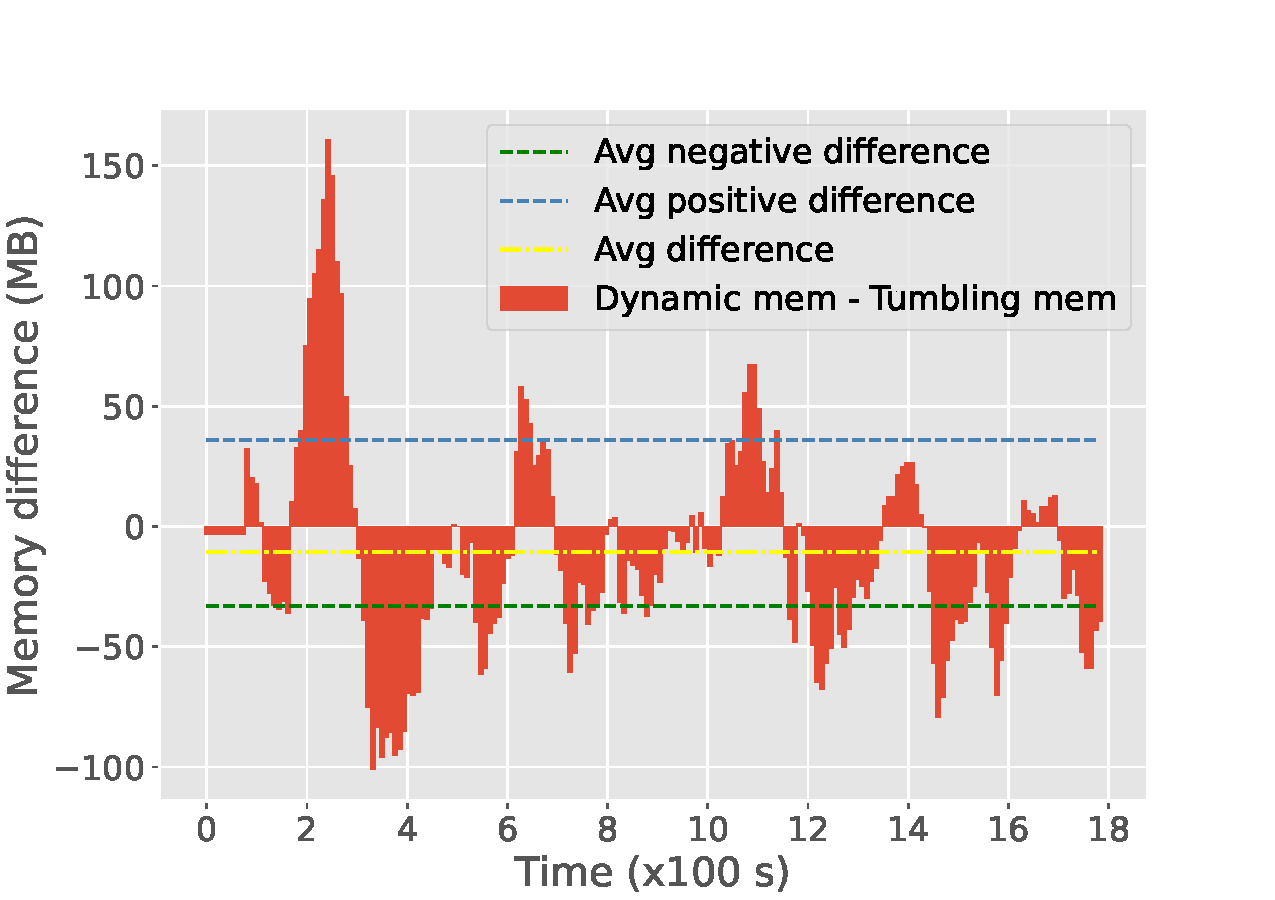
\includegraphics[width=0.5\columnwidth]{fig/periodic/mem_difference_bar.pdf}
        \caption{Relative difference in memory usage from the perspective of dynamic window}
        \label{fig:periodic_mem_diff}
    \end{subfigure}

    \caption[Metrics measurements for periodic workload]
    {Metrics measurements for periodic workload. Dynamic window 
    has lower memory usage on average than Tumbling window for
periodic workload. }%
    \label{fig:periodic_measurement}
\end{figure}

\subsection{Workload for completeness measure}%
\label{sec:Workload for completeness measure}

From the results in Table~\ref{tab:dynamic_completeness}, and 
Table~\ref{tab:tumbling_completeness}, we conclude that Dynamic window 
outperforms Tumbling window in terms of generating a more \emph{complete} output. 
Dynamic window has an IOU score of \textbf{1} for constant low stream rate
due to the subwindow sizes growing large 
enough to accommodate all the required records, to generate the \emph{complete} output set. In contrast, Tumbling window scores only \textbf{0.749}, leading to 
the conclusion that a window size of 2s is not enough to process the low stream rate 
of the evaluation data. 

Similarly for periodic burst input, Dynamic window outperforms Tumbling window with a
score of \textbf{0.982} whereas Tumbling window only scores \textbf{0.780}. The high IOU 
score of Dynamic window is due to its ability  
to adapt to the changing stream rate to hold enough 
records for maximal joined output generation.


\begin{table}[htbp]
    \centering
    \resizebox{0.5\columnwidth}{!}{%
\begin{tabular}{|r|r|}
\hline
\multicolumn{1}{|c|}{Stream rate} & \multicolumn{1}{c|}{\textbf{IOU score}} \\ \hline
Constant rate                                              & \textbf{1}                              \\ \hline
Periodic burst                                        & \textbf{0.982}                          \\ \hline
\end{tabular}%
}
\caption{Dynamic window's completeness measurement.}
\label{tab:dynamic_completeness}
\end{table}

\begin{table}[htbp]
    \centering
    \resizebox{0.5\columnwidth}{!}{%
\begin{tabular}{|r|r|}
\hline
\multicolumn{1}{|c|}{Stream rate} & \multicolumn{1}{c|}{\textbf{IOU score}} \\ \hline
Constant rate       & \textbf{0.749}                              \\ \hline
Periodic burst      & \textbf{0.780}                          \\ \hline
\end{tabular}%
}
\caption{Tumbling window's completeness measurement. }
\label{tab:tumbling_completeness}
\end{table}


\subsection{Summary}%
\label{sec:Result Summary}

In summary, these results show that our implementation of Dynamic window 
provides lower latency, higher throughput, and a more complete 
output than Tumbling window for both 
workloads of constant stream rate, and unstable periodic burst stream rate.

Although memory usage dropped in the workload with periodic burst rate, we 
could not confidently conclude that the Dynamic window effectively used less memory
on average than Tumbling window. The measurement was based on the heap memory of the 
whole evaluation job, not just the window operator. Therefore, there is a need for a 
more precise measurement of memory usage. 

The results for throughput also deviate from those reported by Van Dongen and Van den Poel(2020)~\cite{evalution_of_spe}. 
This is due to the fact that we ran the evaluation using the whole pipeline of RMLStreamer. This incurs some back pressure from the mapping stage, 
causing the throughput of the join stage to stay constant and flat.    

Overall, we could conclude that Dynamic windowing is viable to replace the fixed size 
windows. Especially in use 
cases, where windows are not required to be of fixed size with variable stream rate.  

